
\documentclass[conference]{acmsiggraph}

\TOGonlineid{45678}
\TOGvolume{0}
\TOGnumber{0}
\TOGarticleDOI{1111111.2222222}
\TOGprojectURL{}
\TOGvideoURL{}
\TOGdataURL{}
\TOGcodeURL{}

\title{Real-time shader-based rendering of grass}

\author {Kin Liu\\Manuel Reinfurt}
\pdfauthor{Kin Liu}

\keywords{radiosity, global illumination, constant time}

\begin{document}

\teaser{
  \frame{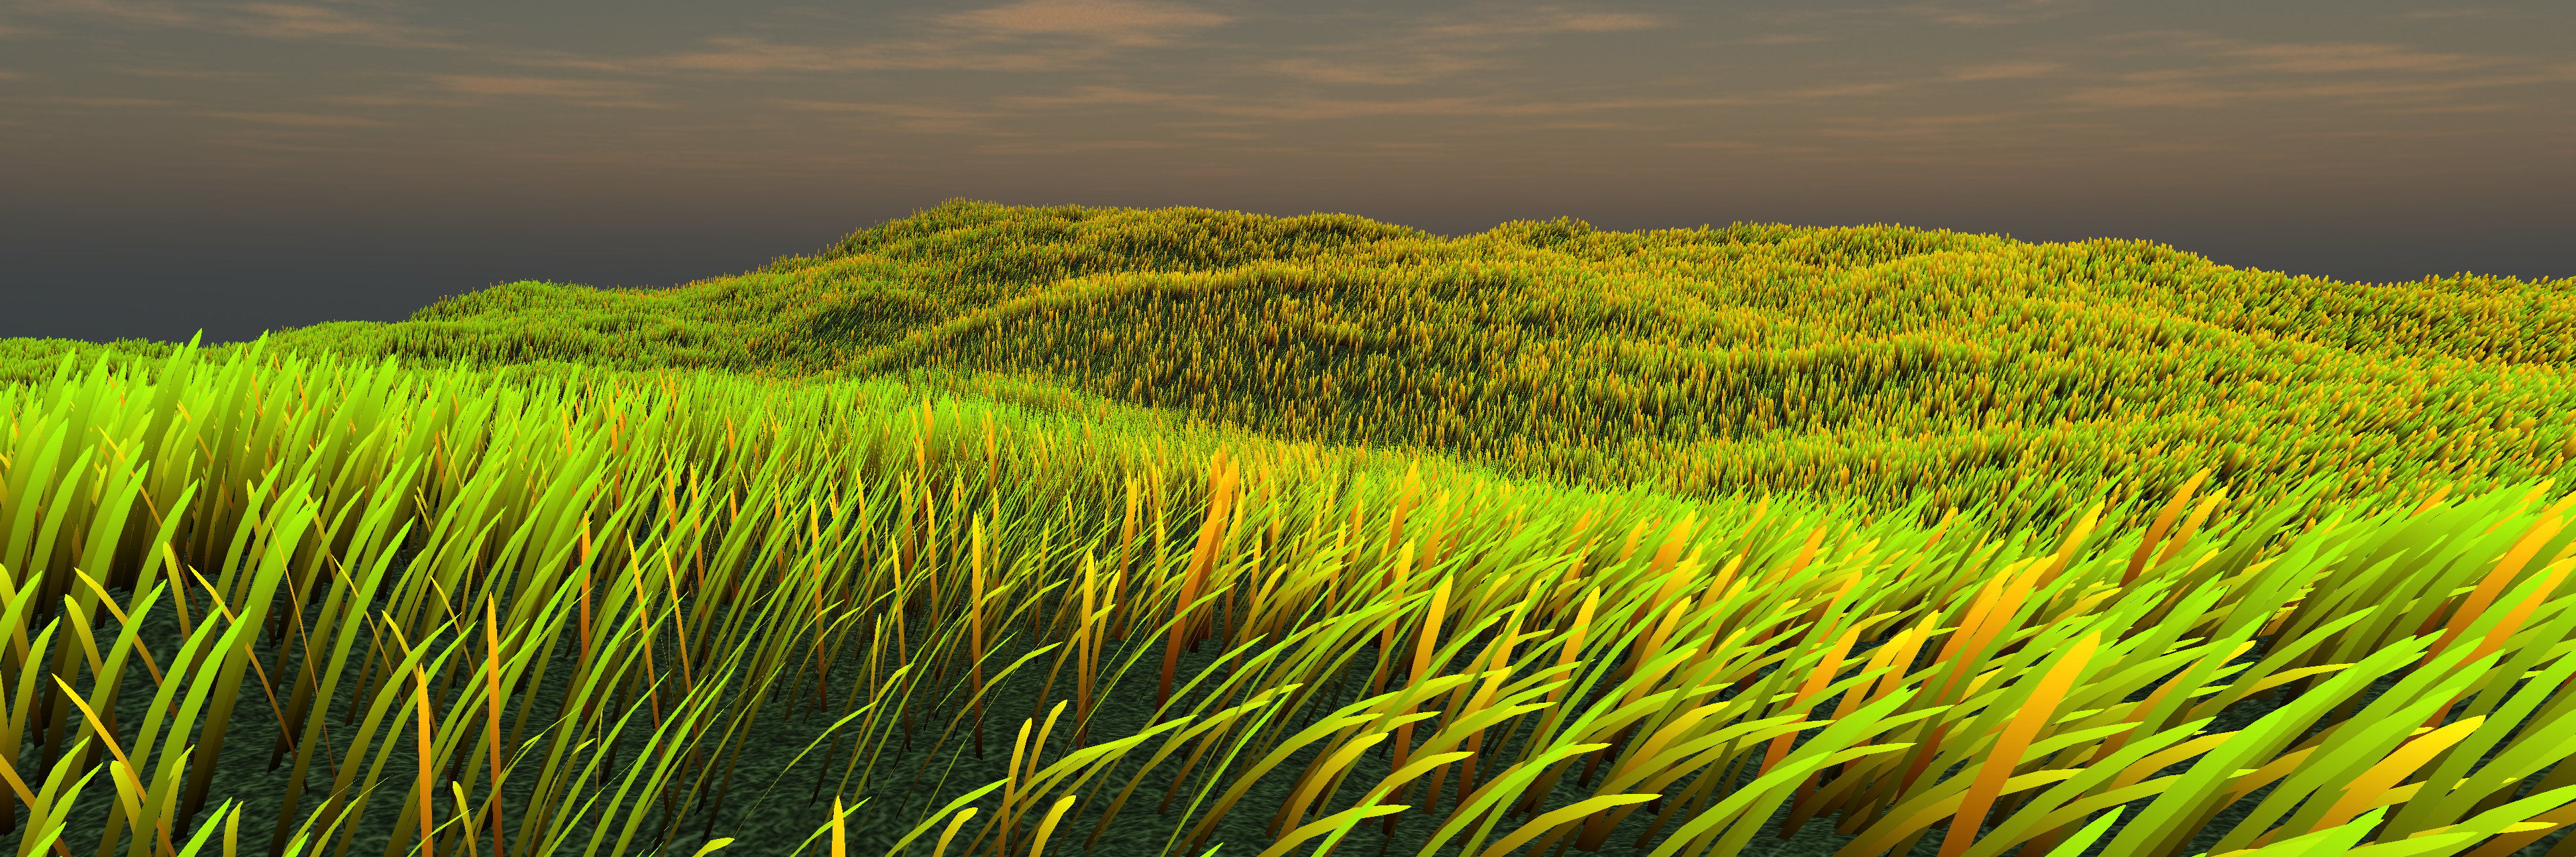
\includegraphics[height=1.5in]{images/final_result}}
  \caption{End result}
}

\maketitle

\begin{abstract}

The grass is the best.

\end{abstract}

\TOGlinkslist

%% Required for all content. 

\copyrightspace

\section{Introduction}

Grass has always been an important factor when it comes to simulate realistic nature scenes. However, due to the sheer amount of individual grass blades and the need to animate them, it is very difficult to implement in real time applications. 

%% \begin{figure}[ht]
%%   \centering
%%   \includegraphics[width=1.5in]{images/samplefigure}
%%   \caption{Sample illustration.}
%% \end{figure}

\section{Related Work}

There are different techniques on how to efficiently and realistically render grass in real time applications. In games, grass is usually simulated by rendering billboards that are laid our in a certain pattern. Animation can be done per vertex, per grass blade or even per cluster. A famous method has been described in GPU Gems 1. While this is a very simple approach that has been used in games for a long time since processing and graphics power is needed elsewhere, it does not yield stunning visuals.

Since DirectX 10, GPUs have been extended with a new shader pipeline - the geometry shader. Using the geometry shader, it is possible to generate grass blades directly on the GPU. This eliminates the CPU as a bottleneck and provides enough power for much more detailed simulations. This paper is based on this approach and combines the work of Eddie Lee (SRC) and ?? (SRC).

The game "Flower", which was released for PlayStation 3, uses this method to render all of its grass. This shows that the approach can be used in real time applications with much success. While the scenes in "Flower" were not really complex and mostly consisted of grass only, the hardware is already very old for todays standards - leaving enough power for more complex scenes which include grass simulation.

\subsection{The Method}
The basic idea is to layout the grass field on the CPU by specifying the root points. This way, the CPU only has to send the position of each single root to the GPU - all other work is done exclusively on the GPU. In order to organize the root points, grass patches are created. Each patch has a certain number of root points and can be controlled individually. The grass patches together then make up the grass grid - which is the grass field.

The grass grid is generated by laying down root points as can be seen in Figure {?}. First, a grid of patches is created and each patch generates its own root points. Using a density map {Figure ?} that is equal the size of the terrain height map, local density spots can be adjusted. All root points are pushed into a single vertex buffer object and can be, in theory, rendered with a single draw call. However, the patches are used to achieve several things:

\begin{description}
  \item[Culling] \hfill \\
  A single patch can be visualized by a bounding box, which can then be easily checked against the view frusrum to cull patches outside of it. It is important to take the grass animation into account when creating the bounding box - otherwise grass could be culled when moving into the frustum.
  \item[Level of detail] \hfill \\
  The distance from the camera to the mid point of a patch can be calculated and used to set the level of detail. This saves a few instructions as level of detail does not have to be calculated within the geometry shader, thus making it possible to use geometry shaders that are pre-compiled with a static vertex count, which will improve performance.
  \item[Further individualization] \hfill \\
	It's possible to pass options into the shaders for rendering a patch, which can be used for wind animation, grass height or any other property of the grass.
\end{description}

\subsection{Terrain}
The terrain is generated out of a height map, which was generated by Perlin Noise. We can map the grass root position to our terrain grid to find the matching Y position. It is important to take the density of the grass into account when calculating lighting of the terrain. Using the density map, we can darken areas where grass is very dense - easily simulating ambient occlusion.

[INSERT picture of terrain with grass on it] (TODO KIN)

\subsection{Generating the blade}
The geometry shader needs to be able to generate grass blades with a different level of detail. Instead of writing separate geometry shaders, we decided to write one geometry shader that prodecurally generates the blade. When generating the blade, we want to concentrate the vertices on the top half of the blade to have a smooth animation later on. It is also needed to calculate the UV-coordinate, normals and rotation, as well as vertex displacement for wind, which is described in chapter 4.

A visual representation of the algorithm can be seen in Figure {?} (TODO MANUEL)

\subsection{Pipeline}
To summarize, this is a list of important components in our project and their respective job.
\begin{description}
  \item[CPU] \hfill \\
  The CPU will generate the root points out of the density map and create a single vertex buffer, that contains all roots. It will also slice the full grass grid into smaller patches, which can be controlled through constant buffers on the GPU.
  
  Since we also have static terrain, the root points will already contain the correct displaced Y position. Additional improvements like culling will also be done on the CPU.
  \item[Vertex shader] \hfill \\
  The vertex shader is, in essence, a pass-through shader.
  \item[Geometry shader] \hfill \\
  All the hard work is done in the geometry shader. Since the geometry shader gets a single point as an input, it's job is to create a grass blade with a specified number of vertices. The geometry shader will also take care of calculating normals, level of detail, and animation.
  \item[Pixel shader] \hfill \\
  To calculate the color, we use the basic Phong BDRF, combined with a texture and a randomized tint.
\end{description}

\subsection{Flickering}
A very prevalent problem while implementing this approach was flickering. Due to the high amount of very thin grass blades, blades were fighting for pixels and a lot of aliasing and flickering could be seen. In order to minimize this effect, several techniques were used:

\begin{description}
  \item[Grass blade proportions] \hfill \\
  Since grass blades far in the distant can not really be distinguished from each other due to having only a few pixels to be displayed, it is possible to increase the width of the grass blades. This way, less blades will be fighting for the pixel - having a clear winner in terms of which color to display, leaves less flickering.
  \item[Density Control] \hfill \\
  Since the goal is to minimize the amount of blades fighting for the pixels, the grass density (number of root points in a patch) can be adjusted depending on the distance to the camera. Combined with the grass blade proportions, this leaves very few grass blades that will fill the space in the distance. However, it should be noted that this approach can lead to grass blades "popping" in and out of the user's view.
  \item[Downsampling] \hfill \\
  The simplest approach is to increase the render target resolution. Rendering the scene at 4k or 8k resolutions and then downsampling it to Full-HD leaves a stunningly clear and flicker-free image behind. While being simple to implement and having very good results, it has the highest performance cost. 
\end{description}

\section{Randomization}

The scene looks very artificial if the grass is laid out with exact distances, when each grass blade has the same tint, height or width. However, it is fairly difficult to generate random numbers on the GPU, which is why we have to use certain tricks to have fairly random grass properties. When laying out the root points, we can generate random positions using the CPU.

Since these root points are given to the geometry shader, and we kow that these positions are random, we can generate a random number between -1 and 1 using the following equation.

\begin{equation}
r = sin(\frac{\pi}2 * frac(root.x) + \frac{\pi}2 * frac(root.z))
\end{equation}

[INSERT non-randomized and randomized picture]

Using this randomized value, several grass properties can be influenced. Some of those are: width, height, color tint, rotation, wind effect.

\section{Animation}
For animating the grass blades, a simulation of wind is used to achieve a realistic look. In order to maximize the interactivity, the user should be able to influence wind speed and direction. 

In general, the wind simulation consists of two components:

\begin{description}
  \item[Vertex displacement] \hfill \\
  This components takes care of simulation the effect of wind hitting a single blade, which displaces the mesh.
  \item[Wind field simulation] \hfill \\
  To simulate the effect of wind over a field of grass, a 2D wind field is used.
\end{description}

\subsection{Vertex displacement}


\subsection{Wind field simulation}

\section{Benchmarks}
We kept randomized values to a minimum to avoid variations in the scene and to have a baseline. All tests were mainly done on the following two systems.

\begin{flushleft}
\begin{description}
  \item[System 1 (Desktop)] \hfill \\
  CPU: Intel Xeon E5-1230v3 \linebreak
  RAM: 8GB DDR3-1333 \linebreak
  GPU: nVidia GeForce GTX 780
  \item[System 2 (Notebook)] \hfill \\
  CPU: Intel Core I7-4980HQ \linebreak
  RAM: 16GB DDR3-1333 \linebreak
  GPU: Intel Iris Pro
\end{description}
\end{flushleft}

Content: Show base FPS without performance improvements, then show level of detail, culling and so on.

\section{Shortcomings and improvements}

As shown in the section "Benchmarks", this approach does not need high-end processing power as of todays standards. Using 1 million grass blades, the implementation can be run on integrated graphics cards on Notebooks with 60 FPS.

The main visual problem is flickering. Using native resolution of displays and no anti-aliasing, the thin blades cause a lot of flickering in the distance - even when using the tricks described in the paper to minimize it. However, when rendered on a high PPI screen or by using techniques like Downsampling, flickering vanishes very fast.

\bibliographystyle{acmsiggraph}
\bibliography{template}
\end{document}
